\section{eo\-Reduce\-Merge\-Reduce$<$ EOT $>$ Class Template Reference}
\label{classeo_reduce_merge_reduce}\index{eoReduceMergeReduce@{eoReduceMergeReduce}}
eo\-Reduce\-Merge\-Reduce is an {\bf eo\-Replacement}{\rm (p.\,\pageref{classeo_replacement})}: - saves possible elite parents - reduces rest of parents - reduces offspring - merges reduced populations - reduces resulting merged pop if necessary  


{\tt \#include $<$eo\-Reduce\-Merge\-Reduce.h$>$}

Inheritance diagram for eo\-Reduce\-Merge\-Reduce$<$ EOT $>$::\begin{figure}[H]
\begin{center}
\leavevmode
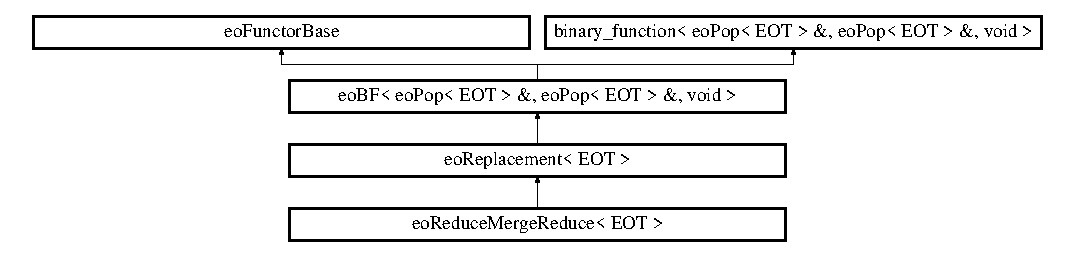
\includegraphics[height=3.01075cm]{classeo_reduce_merge_reduce}
\end{center}
\end{figure}
\subsection*{Public Member Functions}
\begin{CompactItemize}
\item 
{\bf eo\-Reduce\-Merge\-Reduce} ({\bf eo\-How\-Many} \_\-how\-Many\-Elite, bool \_\-strong\-Elitism, {\bf eo\-How\-Many} \_\-how\-Many\-Reduced\-Parents, {\bf eo\-Reduce}$<$ {\bf EOT} $>$ \&\_\-reduce\-Parents, {\bf eo\-How\-Many} \_\-how\-Many\-Reduced\-Offspring, {\bf eo\-Reduce}$<$ {\bf EOT} $>$ \&\_\-reduce\-Offspring, {\bf eo\-Reduce}$<$ {\bf EOT} $>$ \&\_\-reduce\-Final)\label{classeo_reduce_merge_reduce_a0}

\item 
void {\bf operator()} ({\bf eo\-Pop}$<$ {\bf EOT} $>$ \&\_\-parents, {\bf eo\-Pop}$<$ {\bf EOT} $>$ \&\_\-offspring)\label{classeo_reduce_merge_reduce_a1}

\begin{CompactList}\small\item\em The pure virtual function that needs to be implemented by the subclass. \item\end{CompactList}\end{CompactItemize}
\subsection*{Private Attributes}
\begin{CompactItemize}
\item 
{\bf eo\-How\-Many} {\bf how\-Many\-Elite}\label{classeo_reduce_merge_reduce_r0}

\item 
bool {\bf strong\-Elitism}\label{classeo_reduce_merge_reduce_r1}

\item 
{\bf eo\-How\-Many} {\bf how\-Many\-Reduced\-Parents}\label{classeo_reduce_merge_reduce_r2}

\item 
{\bf eo\-How\-Many} {\bf how\-Many\-Reduced\-Offspring}\label{classeo_reduce_merge_reduce_r3}

\item 
{\bf eo\-Reduce}$<$ {\bf EOT} $>$ \& {\bf reduce\-Parents}\label{classeo_reduce_merge_reduce_r4}

\item 
{\bf eo\-Reduce}$<$ {\bf EOT} $>$ \& {\bf reduce\-Offspring}\label{classeo_reduce_merge_reduce_r5}

\item 
{\bf eo\-Reduce}$<$ {\bf EOT} $>$ \& {\bf reduce\-Final}\label{classeo_reduce_merge_reduce_r6}

\end{CompactItemize}


\subsection{Detailed Description}
\subsubsection*{template$<$class EOT$>$ class eo\-Reduce\-Merge\-Reduce$<$ EOT $>$}

eo\-Reduce\-Merge\-Reduce is an {\bf eo\-Replacement}{\rm (p.\,\pageref{classeo_replacement})}: - saves possible elite parents - reduces rest of parents - reduces offspring - merges reduced populations - reduces resulting merged pop if necessary 



Definition at line 49 of file eo\-Reduce\-Merge\-Reduce.h.

The documentation for this class was generated from the following file:\begin{CompactItemize}
\item 
eo\-Reduce\-Merge\-Reduce.h\end{CompactItemize}
